\documentclass[tikz,border=4pt]{standalone}
\usepackage{tikz}
\usetikzlibrary{positioning,arrows.meta,fit,backgrounds,calc,patterns,shapes.geometric,shapes.symbols}

\definecolor{ctrlFill}{HTML}{dae8fc}
\definecolor{ctrlStroke}{HTML}{6c8ebf}
\definecolor{memFill}{HTML}{ffe6cc}
\definecolor{memStroke}{HTML}{d79b00}
\definecolor{calcFill}{HTML}{cce5ff}
\definecolor{calcStroke}{HTML}{4a86e8}
\definecolor{dataFill}{HTML}{d5e8d4}
\definecolor{dataStroke}{HTML}{82b366}
\definecolor{newStroke}{HTML}{b85450}
\definecolor{dramStroke}{HTML}{666666}
\definecolor{streamColor}{HTML}{d79b00}
\definecolor{compColor}{HTML}{4a86e8}

\begin{document}
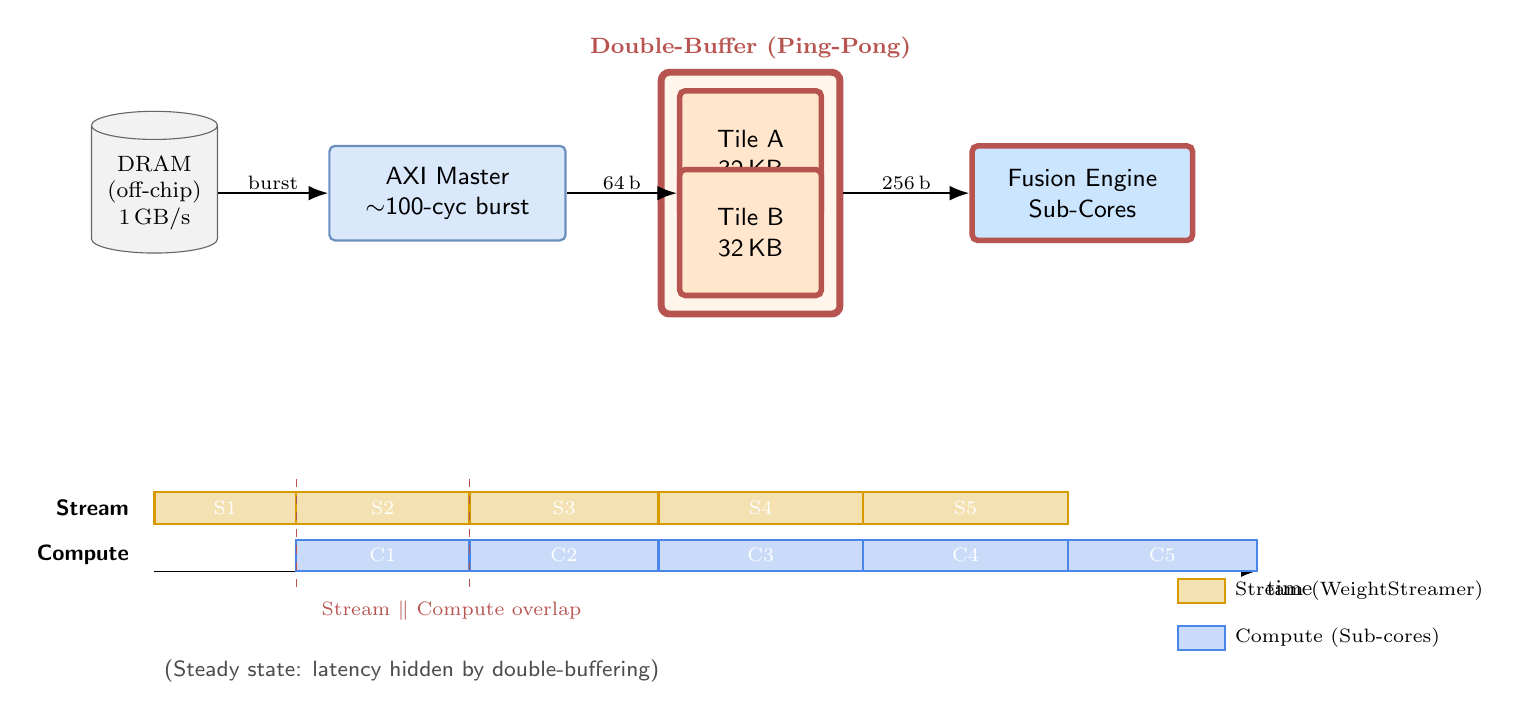
\begin{tikzpicture}[
  font=\small\sffamily,
  dram/.style  ={draw=dramStroke, fill=gray!10, cylinder, shape border rotate=90, aspect=0.25, minimum height=18mm, minimum width=16mm, align=center, font=\footnotesize},
  axi/.style   ={draw=ctrlStroke, fill=ctrlFill, rounded corners=2pt, thick, minimum height=12mm, minimum width=30mm, align=center},
  dbuf/.style  ={draw=newStroke, fill=memFill, rounded corners=2pt, line width=2pt, minimum height=16mm, align=center},
  core/.style  ={draw=newStroke, fill=calcFill, rounded corners=2pt, line width=2pt, minimum height=12mm, minimum width=28mm, align=center},
  arr/.style   ={-{Latex[length=2.5mm]}, thick},
  barstream/.style={draw=streamColor, fill=streamColor!30, thick},
  barcomp/.style  ={draw=compColor,   fill=compColor!30,   thick},
  lbl/.style   ={font=\scriptsize, inner sep=1pt},
]

% ==================== UPPER: hardware pipeline ====================
\node[dram] (dram) at (0,0) {DRAM\\(off-chip)\\1\,GB/s};

\node[axi, right=14mm of dram] (axi) {AXI Master\\$\sim$100-cyc burst};

% Double buffer: Tile A / Tile B
\node[dbuf, minimum width=18mm, right=14mm of axi, yshift=5mm]  (tA) {Tile A\\32\,KB};
\node[dbuf, minimum width=18mm, right=14mm of axi, yshift=-5mm] (tB) {Tile B\\32\,KB};
\begin{pgfonlayer}{background}
  \node[draw=newStroke, line width=2.5pt, rounded corners=3pt, fit=(tA)(tB), inner sep=2mm, fill=memFill!40] (db) {};
  \node[anchor=south, font=\footnotesize\bfseries, text=newStroke] at (db.north) {Double-Buffer (Ping-Pong)};
\end{pgfonlayer}

\node[core, right=16mm of db] (cores) {Fusion Engine\\Sub-Cores};

% Arrows
\draw[arr] (dram.east) -- node[lbl, above]{burst} (axi.west);
\draw[arr] (axi.east) -- node[lbl, above]{64\,b} ($(tA.west)!0.5!(tB.west)$);
\draw[arr] (db.east) -- node[lbl, above]{256\,b} (cores.west);

% ==================== LOWER: Gantt-style timing ====================
\begin{scope}[shift={(0,-48mm)}]
  % Axis
  \draw[-{Latex[length=2mm]}] (0,0) -- (140mm,0) node[below right, font=\footnotesize]{time};
  % Row labels
  \node[anchor=east, font=\footnotesize\sffamily\bfseries] at (-2mm, 8mm) {Stream};
  \node[anchor=east, font=\footnotesize\sffamily\bfseries] at (-2mm, 2mm) {Compute};

  % Bars parameters
  % s_start, s_dur  (stream)
  % c_start, c_dur  (compute) -- starts when stream of this stage done
  \def\barh{4mm}

  % S1
  \fill[barstream] (0mm, 6mm) rectangle ++(18mm, \barh);
  \node[lbl, white] at (9mm, 8mm) {S1};
  \fill[barcomp] (18mm, 0mm) rectangle ++(22mm, \barh);
  \node[lbl, white] at (29mm, 2mm) {C1};

  % S2
  \fill[barstream] (18mm, 6mm) rectangle ++(22mm, \barh);
  \node[lbl, white] at (29mm, 8mm) {S2};
  \fill[barcomp] (40mm, 0mm) rectangle ++(24mm, \barh);
  \node[lbl, white] at (52mm, 2mm) {C2};

  % S3
  \fill[barstream] (40mm, 6mm) rectangle ++(24mm, \barh);
  \node[lbl, white] at (52mm, 8mm) {S3};
  \fill[barcomp] (64mm, 0mm) rectangle ++(26mm, \barh);
  \node[lbl, white] at (77mm, 2mm) {C3};

  % S4
  \fill[barstream] (64mm, 6mm) rectangle ++(26mm, \barh);
  \node[lbl, white] at (77mm, 8mm) {S4};
  \fill[barcomp] (90mm, 0mm) rectangle ++(26mm, \barh);
  \node[lbl, white] at (103mm, 2mm) {C4};

  % S5
  \fill[barstream] (90mm, 6mm) rectangle ++(26mm, \barh);
  \node[lbl, white] at (103mm, 8mm) {S5};
  \fill[barcomp] (116mm, 0mm) rectangle ++(24mm, \barh);
  \node[lbl, white] at (128mm, 2mm) {C5};

  % Overlap shading brackets
  \draw[dashed, newStroke] (18mm, -2mm) -- (18mm, 12mm);
  \draw[dashed, newStroke] (40mm, -2mm) -- (40mm, 12mm);
  \node[text=newStroke, font=\scriptsize, anchor=west] at (20mm, -5mm) {Stream $\parallel$ Compute overlap};

  \node[anchor=north west, font=\footnotesize\sffamily, text=black!70] at (0,-10mm) {(Steady state: latency hidden by double-buffering)};
\end{scope}

% ==================== Legend ====================
\begin{scope}[shift={(130mm, -58mm)}]
  \fill[barstream] (0,6mm) rectangle ++(6mm,3mm); \node[right, font=\scriptsize] at (6mm, 7.5mm) {Stream (WeightStreamer)};
  \fill[barcomp]   (0,0mm) rectangle ++(6mm,3mm); \node[right, font=\scriptsize] at (6mm, 1.5mm) {Compute (Sub-cores)};
\end{scope}

\end{tikzpicture}
\end{document}
